\documentclass[aspectratio=169]{beamer}

\usetheme{Boadilla}
\usecolortheme{dolphin}
\setbeamertemplate{navigation symbols}{}
\setbeamertemplate{footline}[frame number]

\usepackage{amsmath,amssymb}
\usepackage{graphicx}
\usepackage{booktabs}

\graphicspath{{../../output/model/}{../../output/graphs/}}

\title[AI \& Labor Market Risk]{Present Day, Present Time:\\
  AI Exposure and Labor Market Risk}
\author{Leyao Wang}
\institute{University of Virginia \\ ECON 4210 --- International Trade}
\date{March 2026}

% ── Color helpers ──────────────────────────────────────────────────────────────
\definecolor{myblue}{RGB}{33,102,172}
\definecolor{myred}{RGB}{215,48,39}
\definecolor{mygreen}{RGB}{26,150,65}

\begin{document}

\begin{frame}
\titlepage
\end{frame}

% =============================================================================
% SLIDE 1 — Inspiration
% =============================================================================
\begin{frame}{Where the Model Comes From}

\textbf{Two papers from trade economics:}

\bigskip
\begin{columns}[t]
\column{0.48\textwidth}
  \textbf{Grossman \& Rossi-Hansberg (2008)}\\[4pt]
  \textit{``Trading Tasks''}
  \begin{itemize}
    \item Production $=$ a bundle of tasks, not just inputs
    \item Some tasks can be \emph{offshored} cheaply; others can't
    \item A falling ``offshoring cost'' $\rightarrow$ more tasks sent abroad
    \item Workers in offshored tasks face wage pressure
  \end{itemize}

\column{0.48\textwidth}
  \textbf{Ottaviano, Peri \& Wright (2013)}\\[4pt]
  \textit{Immigration, Offshoring, and American Jobs}
  \begin{itemize}
    \item Extends GRH: workers differ in \emph{type} $i^*$
    \item Different worker groups face different offshoring cutoffs
    \item Heterogeneous exposure across the wage distribution
  \end{itemize}
\end{columns}

\bigskip\hrule\bigskip

\textbf{Why does this map to AI?}\\[4pt]
Offshoring delegates tasks to cheaper foreign labor.
AI delegates tasks to a cheaper \emph{technology}.
The mechanism is the same: a cost shifter that undercuts some tasks but not others.

\end{frame}

% =============================================================================
% SLIDE 2 — Model Setup
% =============================================================================
\begin{frame}{Model Setup}

\textbf{Tasks, workers, and production}

\medskip
\begin{itemize}
  \item Cognitive tasks indexed $i \in [0,1]$ by AI susceptibility
  \begin{itemize}
    \item Low $i$ = routine cognitive (data entry, drafting, coding) --- easy for AI
    \item High $i$ = complex, judgment-intensive --- hard for AI
  \end{itemize}

  \medskip
  \item Final output aggregates tasks via \textbf{CES technology}:
  \[
    Y = \left[\int_0^1 y(i)^{\frac{\sigma-1}{\sigma}}\,di\right]^{\!\frac{\sigma}{\sigma-1}}
  \]

  \medskip
  \item \textbf{Workers:} each worker type $i^*$ specializes in task $i^*$;
        supply of task $i$ is $f(i)$ (fixed, inelastic)

  \medskip
  \item \textbf{AI cost} of performing task $i$:
  \[
    c^{\mathrm{AI}}(i) = \tau \cdot e^{\alpha i}, \quad \tau > 0,\;\alpha > 0
  \]
  Lower $\tau$ = more capable AI. \quad $e^{\alpha i}$ rises steeply --- complex tasks stay expensive for AI.

  \medskip
  \item Firms are competitive; output price $P_Y$ is fixed (small open economy)
\end{itemize}

\end{frame}

% =============================================================================
% SLIDE 3 — Pre-AI Equilibrium
% =============================================================================
\begin{frame}{Pre-AI Equilibrium: Wages Follow Task Prices}

\textbf{Step 1 — Firm cost minimization gives task demand:}
\[
  y^d(i) = Y \cdot \left(\frac{P_Y}{p_0(i)}\right)^{\!\sigma}
\]

\textbf{Step 2 — Market clearing} $\bigl(y^d(i) = f(i)\bigr)$ pins down the equilibrium task price:
\[
  \boxed{p_0(i) = P_Y \cdot \left(\frac{Y}{f(i)}\right)^{\!1/\sigma}}
\]

\textbf{Step 3 — Under full specialization, each worker earns their task price:}
\[
  w_0(i^*) = p_0(i^*)
\]

\bigskip
\begin{columns}[c]
\column{0.55\textwidth}
  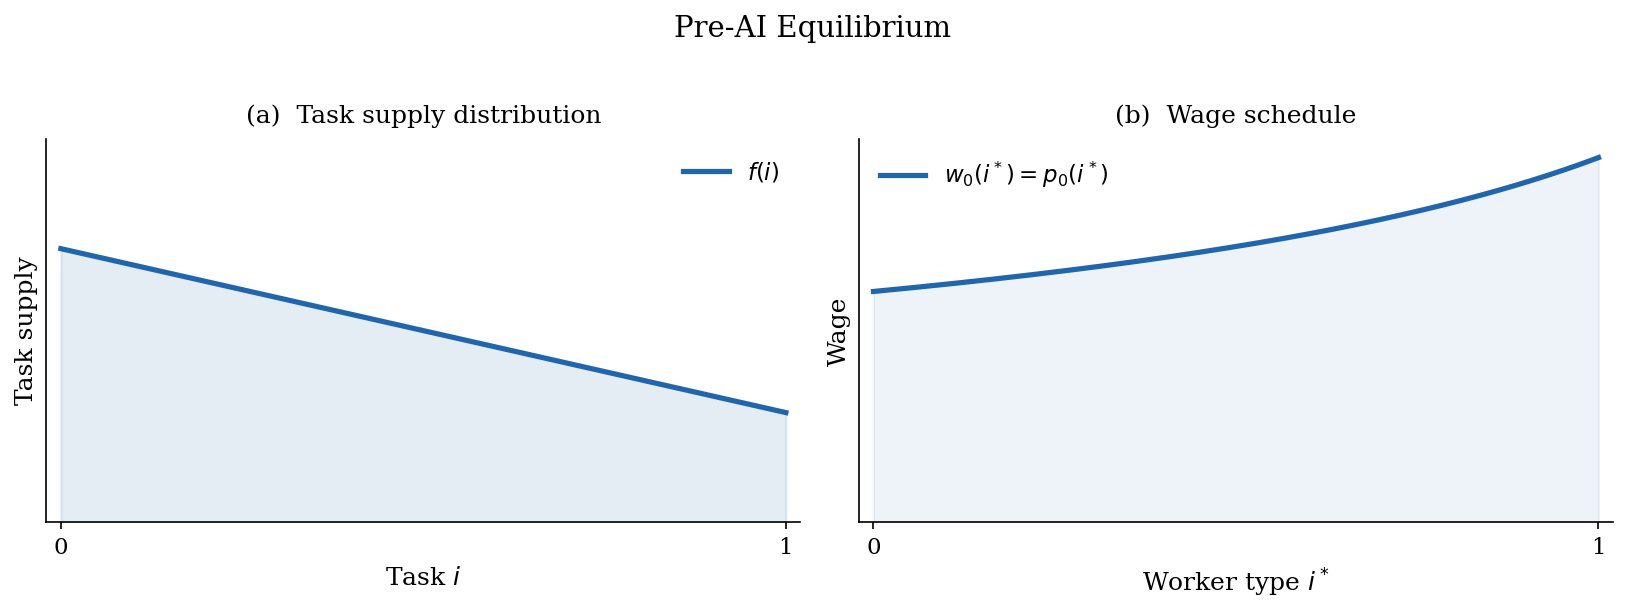
\includegraphics[width=\linewidth]{fig_preai.png}
\column{0.42\textwidth}
  \small
  The wage schedule $w_0(i^*)$ reflects how scarce each worker type is relative to how much the firm values that task.\\[6pt]
  \textit{(Upward slope is for illustration --- the model imposes no restriction on the shape of $p_0$.)}
\end{columns}

\end{frame}

% =============================================================================
% SLIDE 4 — Post-AI Shock
% =============================================================================
\begin{frame}{Post-AI Shock: The Automation Cutoff}

\textbf{AI enters as a competing supplier.} Competition drives task prices to:
\[
  p(i) = \min\!\bigl(p_0(i),\;\tau e^{\alpha i}\bigr)
\]

\textbf{An automation cutoff $I^*$ emerges} where AI cost = pre-AI task price:
\[
  \tau\, e^{\alpha I^*} = p_0(I^*)
\]

\begin{columns}[c]
\column{0.55\textwidth}
  
\includegraphics[width=\linewidth]{fig_postai.png}
\column{0.42\textwidth}
  \small
  \begin{itemize}
    \item Tasks $i < I^*$: AI undercuts $\rightarrow$ \textcolor{myred}{wage compression}
    \[
      \Delta w(i^*) = \tau e^{\alpha i^*} - p_0(i^*) < 0
    \]
    \item Tasks $i \geq I^*$: human price prevails $\rightarrow$ \textcolor{mygreen}{unaffected}
    \item If compressed wage $<$ reservation wage $\rightarrow$ \textbf{unemployment}
  \end{itemize}
\end{columns}

\bigskip
{\small\textit{The sign of $\Delta w < 0$ is unambiguous for all $i^* < I^*$: by definition of the cutoff, AI cost lies strictly below the pre-AI price throughout the automated range.}}

\end{frame}

% =============================================================================
% SLIDE 5 — More on I*
% =============================================================================
\begin{frame}{What Determines the Cutoff $I^*$?}

\begin{columns}[t]
\column{0.50\textwidth}

  \textbf{As AI improves ($\tau \downarrow$), $I^*$ rises}\\[4pt]
  The automation frontier expands toward more complex tasks.
  Formally:
  \[
    \frac{\partial I^*}{\partial \tau} < 0
  \]

  \medskip
  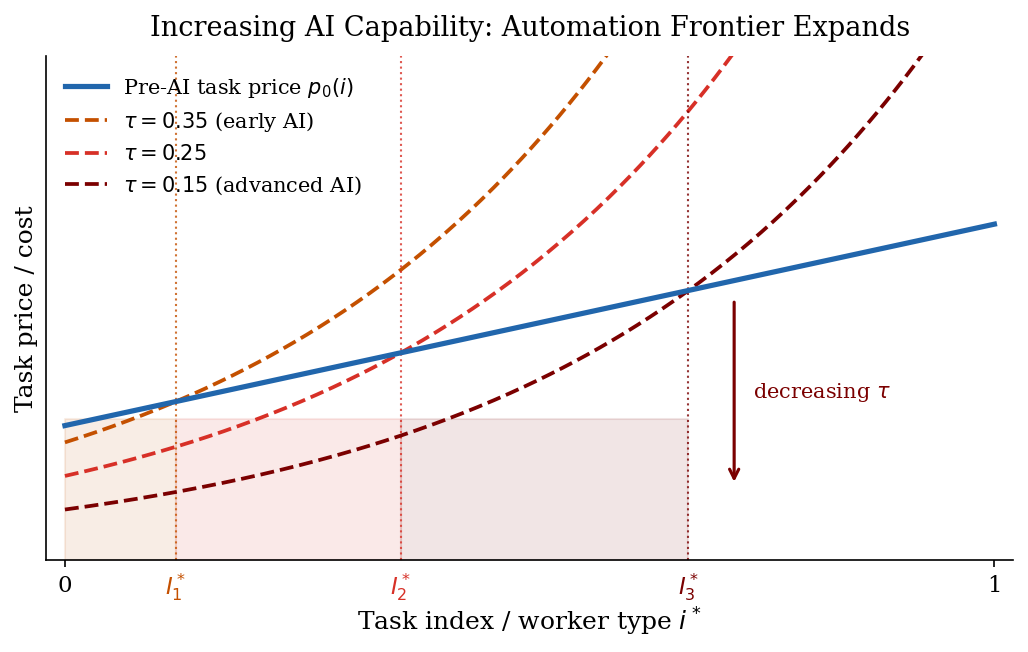
\includegraphics[width=\linewidth]{fig_capability.png}
  \vspace{-4pt}
  {\tiny Decreasing $\tau$ shifts the AI cost curve down, pushing $I^*$ rightward.}

\column{0.48\textwidth}

  \textbf{What if $p_0(i)$ is non-monotone?}\\[4pt]
  The cutoff may not be unique --- the automated set becomes a \emph{union of intervals}:
  \[
    \mathcal{A} = [0, I_1^*] \cup [I_2^*, I_3^*] \cup \cdots
  \]

  \medskip
  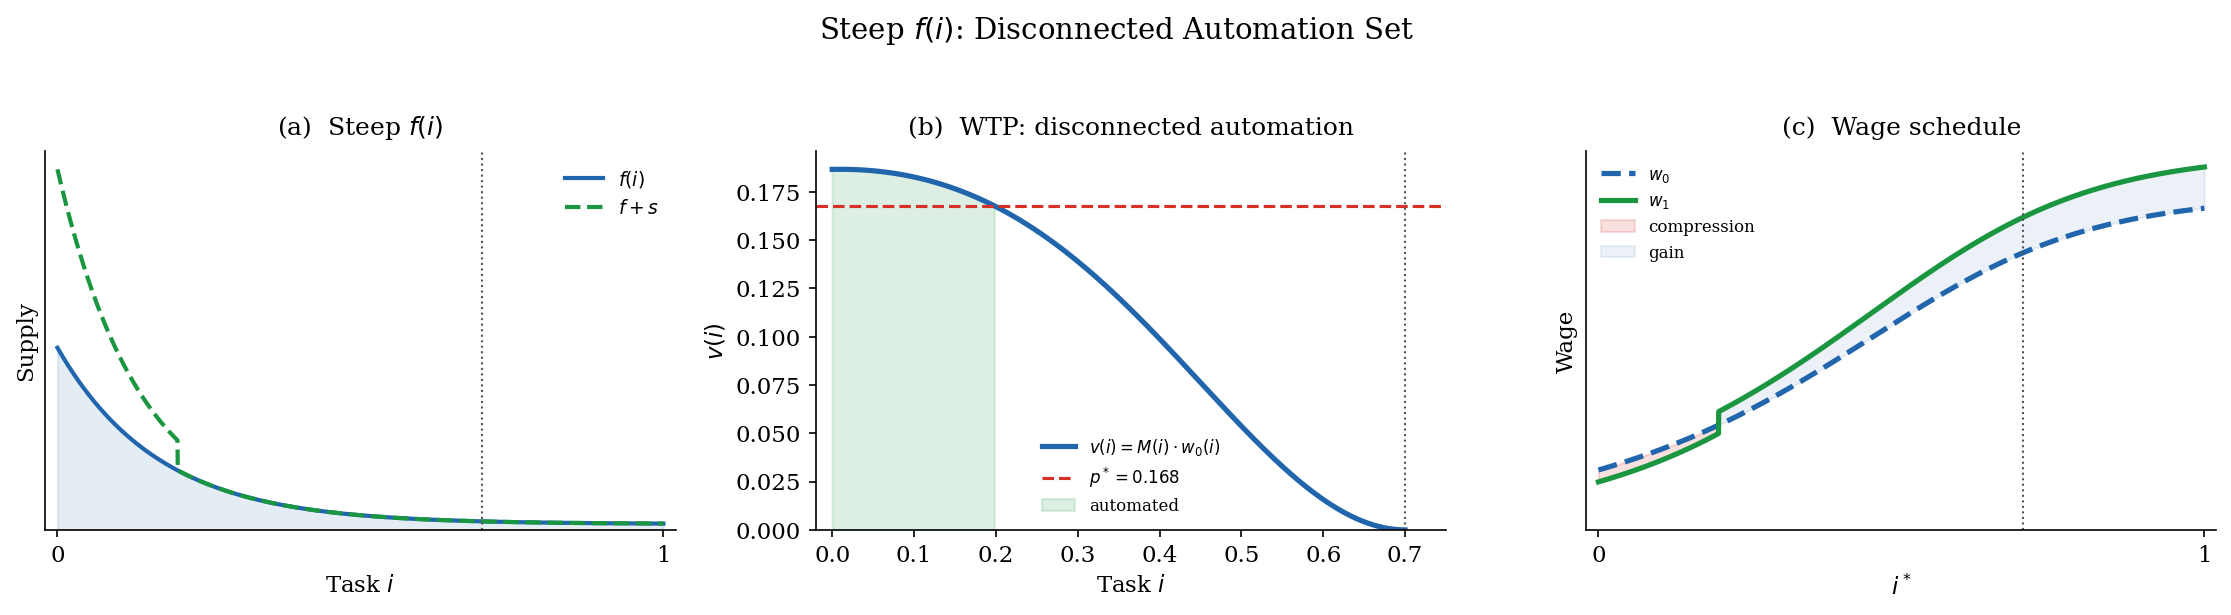
\includegraphics[width=\linewidth]{fig_multiple.png}
  \vspace{-4pt}
  {\tiny Wage compression still applies to all $i^* \in \mathcal{A}$; exposed workers are not necessarily concentrated at the low end.}

\end{columns}

\end{frame}

% =============================================================================
% SLIDE 6 — Empirical Teaser
% =============================================================================
\begin{frame}{Do We See This in the Data?}

\textbf{Unemployment $\times$ AI Exposure (CPS-ASEC, 2018--2025)}

\bigskip
\begin{columns}[c]
\column{0.62\textwidth}
  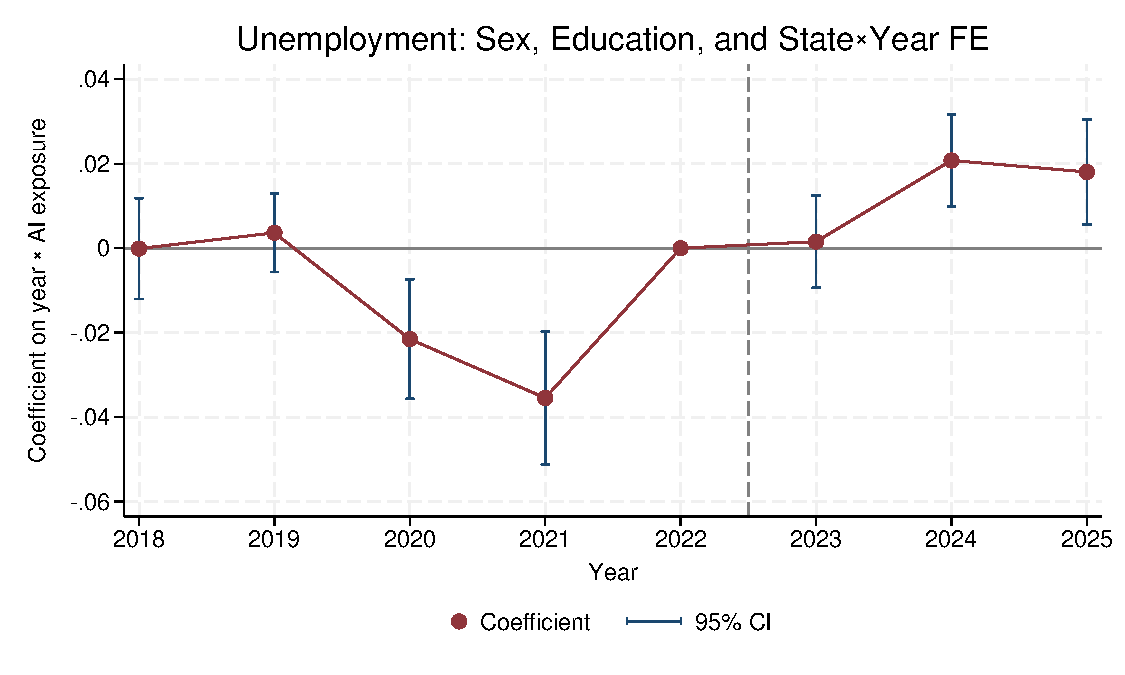
\includegraphics[width=\linewidth]{unemployment_stateYFE_plot.pdf}
\column{0.36\textwidth}
  \small
  \begin{itemize}
    \item DiD design: compares workers in high vs.\ low AI-exposure occupations, before vs.\ after ChatGPT (2022)
    \item Year 2022 = baseline
    \item \textbf{Post-2022}: higher-exposure workers show rising unemployment relative to low-exposure workers
    \item Consistent with the model: workers below $I^*$ face displacement
  \end{itemize}
\end{columns}

\bigskip
{\small\textit{Full estimation details in the paper. The pattern is stable across specifications.}}

\end{frame}

% =============================================================================
% THANK YOU
% =============================================================================
\begin{frame}{}
\centering
\vspace{2cm}
{\Large Thank you!}\\[1.5cm]
{\normalsize Questions welcome.}\\[0.5cm]
{\small \textit{Present Day, Present Time: AI Exposure and Labor Market Risk}}\\
{\small Leyao Wang --- University of Virginia}
\end{frame}

\end{document}
